\documentclass{ximera}

%\usepackage{todonotes}

\newcommand{\todo}{}

\usepackage{esint} % for \oiint
\ifxake%%https://math.meta.stackexchange.com/questions/9973/how-do-you-render-a-closed-surface-double-integral
\renewcommand{\oiint}{{\large\bigcirc}\kern-1.56em\iint}
\fi


\graphicspath{
  {./}
  {ximeraTutorial/}
  {basicPhilosophy/}
  {functionsOfSeveralVariables/}
  {normalVectors/}
  {lagrangeMultipliers/}
  {vectorFields/}
  {greensTheorem/}
  {shapeOfThingsToCome/}
  {dotProducts/}
  {partialDerivativesAndTheGradientVector/}
  {../productAndQuotientRules/exercises/}
  {../normalVectors/exercisesParametricPlots/}
  {../continuityOfFunctionsOfSeveralVariables/exercises/}
  {../partialDerivativesAndTheGradientVector/exercises/}
  {../directionalDerivativeAndChainRule/exercises/}
  {../commonCoordinates/exercisesCylindricalCoordinates/}
  {../commonCoordinates/exercisesSphericalCoordinates/}
  {../greensTheorem/exercisesCurlAndLineIntegrals/}
  {../greensTheorem/exercisesDivergenceAndLineIntegrals/}
  {../shapeOfThingsToCome/exercisesDivergenceTheorem/}
  {../greensTheorem/}
  {../shapeOfThingsToCome/}
  {../separableDifferentialEquations/exercises/}
  {vectorFields/}
}

\newcommand{\mooculus}{\textsf{\textbf{MOOC}\textnormal{\textsf{ULUS}}}}

\usepackage{tkz-euclide}
\usepackage{tikz}
\usepackage{tikz-cd}
\usetikzlibrary{arrows}
\tikzset{>=stealth,commutative diagrams/.cd,
  arrow style=tikz,diagrams={>=stealth}} %% cool arrow head
\tikzset{shorten <>/.style={ shorten >=#1, shorten <=#1 } } %% allows shorter vectors

\usetikzlibrary{backgrounds} %% for boxes around graphs
\usetikzlibrary{shapes,positioning}  %% Clouds and stars
\usetikzlibrary{matrix} %% for matrix
\usepgfplotslibrary{polar} %% for polar plots
\usepgfplotslibrary{fillbetween} %% to shade area between curves in TikZ
%\usetkzobj{all}
\usepackage[makeroom]{cancel} %% for strike outs
%\usepackage{mathtools} %% for pretty underbrace % Breaks Ximera
%\usepackage{multicol}
\usepackage{pgffor} %% required for integral for loops



%% http://tex.stackexchange.com/questions/66490/drawing-a-tikz-arc-specifying-the-center
%% Draws beach ball
\tikzset{pics/carc/.style args={#1:#2:#3}{code={\draw[pic actions] (#1:#3) arc(#1:#2:#3);}}}



\usepackage{array}
\setlength{\extrarowheight}{+.1cm}
\newdimen\digitwidth
\settowidth\digitwidth{9}
\def\divrule#1#2{
\noalign{\moveright#1\digitwidth
\vbox{\hrule width#2\digitwidth}}}




% \newcommand{\RR}{\mathbb R}
% \newcommand{\R}{\mathbb R}
% \newcommand{\N}{\mathbb N}
% \newcommand{\Z}{\mathbb Z}

\newcommand{\sagemath}{\textsf{SageMath}}


%\renewcommand{\d}{\,d\!}
%\renewcommand{\d}{\mathop{}\!d}
%\newcommand{\dd}[2][]{\frac{\d #1}{\d #2}}
%\newcommand{\pp}[2][]{\frac{\partial #1}{\partial #2}}
% \renewcommand{\l}{\ell}
%\newcommand{\ddx}{\frac{d}{\d x}}

% \newcommand{\zeroOverZero}{\ensuremath{\boldsymbol{\tfrac{0}{0}}}}
%\newcommand{\inftyOverInfty}{\ensuremath{\boldsymbol{\tfrac{\infty}{\infty}}}}
%\newcommand{\zeroOverInfty}{\ensuremath{\boldsymbol{\tfrac{0}{\infty}}}}
%\newcommand{\zeroTimesInfty}{\ensuremath{\small\boldsymbol{0\cdot \infty}}}
%\newcommand{\inftyMinusInfty}{\ensuremath{\small\boldsymbol{\infty - \infty}}}
%\newcommand{\oneToInfty}{\ensuremath{\boldsymbol{1^\infty}}}
%\newcommand{\zeroToZero}{\ensuremath{\boldsymbol{0^0}}}
%\newcommand{\inftyToZero}{\ensuremath{\boldsymbol{\infty^0}}}



% \newcommand{\numOverZero}{\ensuremath{\boldsymbol{\tfrac{\#}{0}}}}
% \newcommand{\dfn}{\textbf}
% \newcommand{\unit}{\,\mathrm}
% \newcommand{\unit}{\mathop{}\!\mathrm}
% \newcommand{\eval}[1]{\bigg[ #1 \bigg]}
% \newcommand{\seq}[1]{\left( #1 \right)}
% \renewcommand{\epsilon}{\varepsilon}
% \renewcommand{\phi}{\varphi}


% \renewcommand{\iff}{\Leftrightarrow}

% \DeclareMathOperator{\arccot}{arccot}
% \DeclareMathOperator{\arcsec}{arcsec}
% \DeclareMathOperator{\arccsc}{arccsc}
% \DeclareMathOperator{\si}{Si}
% \DeclareMathOperator{\scal}{scal}
% \DeclareMathOperator{\sign}{sign}


%% \newcommand{\tightoverset}[2]{% for arrow vec
%%   \mathop{#2}\limits^{\vbox to -.5ex{\kern-0.75ex\hbox{$#1$}\vss}}}
% \newcommand{\arrowvec}[1]{{\overset{\rightharpoonup}{#1}}}
% \renewcommand{\vec}[1]{\arrowvec{\mathbf{#1}}}
% \renewcommand{\vec}[1]{{\overset{\boldsymbol{\rightharpoonup}}{\mathbf{#1}}}}

% \newcommand{\point}[1]{\left(#1\right)} %this allows \vector{ to be changed to \vector{ with a quick find and replace
% \newcommand{\pt}[1]{\mathbf{#1}} %this allows \vec{ to be changed to \vec{ with a quick find and replace
% \newcommand{\Lim}[2]{\lim_{\point{#1} \to \point{#2}}} %Bart, I changed this to point since I want to use it.  It runs through both of the exercise and exerciseE files in limits section, which is why it was in each document to start with.

% \DeclareMathOperator{\proj}{\mathbf{proj}}
% \newcommand{\veci}{{\boldsymbol{\hat{\imath}}}}
% \newcommand{\vecj}{{\boldsymbol{\hat{\jmath}}}}
% \newcommand{\veck}{{\boldsymbol{\hat{k}}}}
% \newcommand{\vecl}{\vec{\boldsymbol{\l}}}
% \newcommand{\uvec}[1]{\mathbf{\hat{#1}}}
% \newcommand{\utan}{\mathbf{\hat{t}}}
% \newcommand{\unormal}{\mathbf{\hat{n}}}
% \newcommand{\ubinormal}{\mathbf{\hat{b}}}

% \newcommand{\dotp}{\bullet}
% \newcommand{\cross}{\boldsymbol\times}
% \newcommand{\grad}{\boldsymbol\nabla}
% \newcommand{\divergence}{\grad\dotp}
% \newcommand{\curl}{\grad\cross}
%\DeclareMathOperator{\divergence}{divergence}
%\DeclareMathOperator{\curl}[1]{\grad\cross #1}
% \newcommand{\lto}{\mathop{\longrightarrow\,}\limits}

% \renewcommand{\bar}{\overline}

\colorlet{textColor}{black}
\colorlet{background}{white}
\colorlet{penColor}{blue!50!black} % Color of a curve in a plot
\colorlet{penColor2}{red!50!black}% Color of a curve in a plot
\colorlet{penColor3}{red!50!blue} % Color of a curve in a plot
\colorlet{penColor4}{green!50!black} % Color of a curve in a plot
\colorlet{penColor5}{orange!80!black} % Color of a curve in a plot
\colorlet{penColor6}{yellow!70!black} % Color of a curve in a plot
\colorlet{fill1}{penColor!20} % Color of fill in a plot
\colorlet{fill2}{penColor2!20} % Color of fill in a plot
\colorlet{fillp}{fill1} % Color of positive area
\colorlet{filln}{penColor2!20} % Color of negative area
\colorlet{fill3}{penColor3!20} % Fill
\colorlet{fill4}{penColor4!20} % Fill
\colorlet{fill5}{penColor5!20} % Fill
\colorlet{gridColor}{gray!50} % Color of grid in a plot

\newcommand{\surfaceColor}{violet}
\newcommand{\surfaceColorTwo}{redyellow}
\newcommand{\sliceColor}{greenyellow}




\pgfmathdeclarefunction{gauss}{2}{% gives gaussian
  \pgfmathparse{1/(#2*sqrt(2*pi))*exp(-((x-#1)^2)/(2*#2^2))}%
}


%%%%%%%%%%%%%
%% Vectors
%%%%%%%%%%%%%

%% Simple horiz vectors
\renewcommand{\vector}[1]{\left\langle #1\right\rangle}


%% %% Complex Horiz Vectors with angle brackets
%% \makeatletter
%% \renewcommand{\vector}[2][ , ]{\left\langle%
%%   \def\nextitem{\def\nextitem{#1}}%
%%   \@for \el:=#2\do{\nextitem\el}\right\rangle%
%% }
%% \makeatother

%% %% Vertical Vectors
%% \def\vector#1{\begin{bmatrix}\vecListA#1,,\end{bmatrix}}
%% \def\vecListA#1,{\if,#1,\else #1\cr \expandafter \vecListA \fi}

%%%%%%%%%%%%%
%% End of vectors
%%%%%%%%%%%%%

%\newcommand{\fullwidth}{}
%\newcommand{\normalwidth}{}



%% makes a snazzy t-chart for evaluating functions
%\newenvironment{tchart}{\rowcolors{2}{}{background!90!textColor}\array}{\endarray}

%%This is to help with formatting on future title pages.
\newenvironment{sectionOutcomes}{}{}



%% Flowchart stuff
%\tikzstyle{startstop} = [rectangle, rounded corners, minimum width=3cm, minimum height=1cm,text centered, draw=black]
%\tikzstyle{question} = [rectangle, minimum width=3cm, minimum height=1cm, text centered, draw=black]
%\tikzstyle{decision} = [trapezium, trapezium left angle=70, trapezium right angle=110, minimum width=3cm, minimum height=1cm, text centered, draw=black]
%\tikzstyle{question} = [rectangle, rounded corners, minimum width=3cm, minimum height=1cm,text centered, draw=black]
%\tikzstyle{process} = [rectangle, minimum width=3cm, minimum height=1cm, text centered, draw=black]
%\tikzstyle{decision} = [trapezium, trapezium left angle=70, trapezium right angle=110, minimum width=3cm, minimum height=1cm, text centered, draw=black]


\title{Direction Vectors}

\begin{document}

\begin{abstract}
unit vectors
\end{abstract}
\maketitle




On the real number line, we draw ``tick'' marks to mark off distances of $1$ to the left and right of $0$. On the real number line, we have two direction vectors: $-1$ and $1$.  They establish a unit length in each direction. Every real number is a positive scalar multiple of one of these.

Can we do the same thing for the Complex numbers? \\









\begin{definition}  \textbf{\textcolor{green!50!black}{Direction Vectors}}   \\

A \textbf{direction vector}, also called a \textbf{unit vector}, is a vector of length $1$.

\end{definition}









$\blacktriangleright$ \textbf{\textcolor{blue!75!black}{Polar(Circular) Coordinates}}  \\


Of course, this is easy with polar coordinates.  Unit vectors look like $(1, \theta)$. \\

Every complex number can be described as a positive scalar multiple of a polar unit vector:  


\[
r \cdot (1, \theta) = (r, 0) \cdot (1, \theta) = (r, \theta)
\]



\begin{center}
\textbf{\textcolor{red!80!black}{How can we do this with rectangular coordinates?}}
\end{center}



Can we describe each complex number as a scalar multiple of a unit vector in rectangular coordinates? \\






$\blacktriangleright$ \textbf{\textcolor{blue!75!black}{Rectangular Coordinates}}  


Currently, we can describe every complex number as a sum of two scalar multiples of two direction vectors: 

\[ \hat{x} = \langle 1, 0 \rangle  \, \text{ and }  \, \hat{y} = \langle 0, 1 \rangle      \]


The Cartesian plane has two axes, so two sets of tick marks on two lines.  The left/right tick marks are marking off multiples of $\langle 1, 0 \rangle$ on the real axis. The up/down tick marks are marking off multiples of $\langle 0, 1 \rangle$ on the imaginary axis.




We can view our vectors as constructed as a sum of perpendicular pieces, each of size $1$.



\begin{example}


\[ \langle 5, 7 \rangle = 5 \cdot  \langle 1, 0 \rangle + 7 \cdot \langle 0, 1 \rangle  \]









\begin{image}
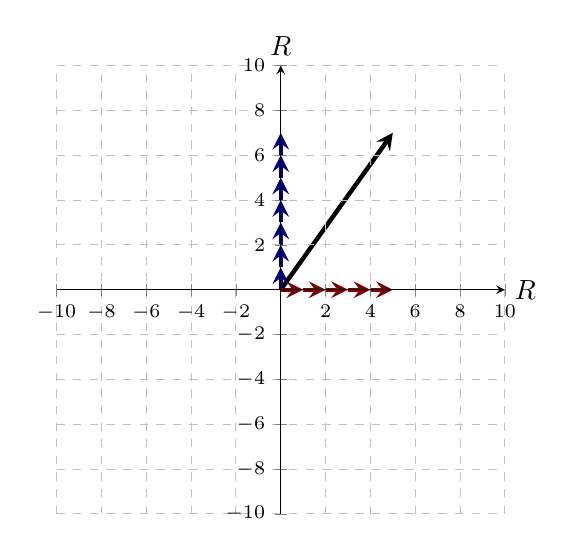
\begin{tikzpicture}
  \begin{axis}[
            domain=-10:10, ymax=10, xmax=10, ymin=-10, xmin=-10,
            axis lines =center, xlabel=$\mathbb{R}$, ylabel=$\mathbb{R}$, grid = major, grid style={dashed},
            unit vector ratio*=1 1 1,
            ytick={-10,-8,-6,-4,-2,2,4,6,8,10},
            xtick={-10,-8,-6,-4,-2,2,4,6,8,10},
            ticklabel style={font=\scriptsize},
            every axis y label/.style={at=(current axis.above origin),anchor=south},
            every axis x label/.style={at=(current axis.right of origin),anchor=west},
            axis on top
          ]
          

          \draw[black,ultra thick,->] (axis cs:0,0) -- (axis cs:5,7);

          \draw[penColor,ultra thick,->] (axis cs:0,0) -- (axis cs:0,1);
          \draw[penColor,ultra thick,->] (axis cs:0,1) -- (axis cs:0,2);
          \draw[penColor,ultra thick,->] (axis cs:0,2) -- (axis cs:0,3);
          \draw[penColor,ultra thick,->] (axis cs:0,3) -- (axis cs:0,4);
          \draw[penColor,ultra thick,->] (axis cs:0,4) -- (axis cs:0,5);
          \draw[penColor,ultra thick,->] (axis cs:0,5) -- (axis cs:0,6);
          \draw[penColor,ultra thick,->] (axis cs:0,6) -- (axis cs:0,7);



          \draw[penColor2,ultra thick,->] (axis cs:0,0) -- (axis cs:1,0);
          \draw[penColor2,ultra thick,->] (axis cs:1,0) -- (axis cs:2,0);
          \draw[penColor2,ultra thick,->] (axis cs:2,0) -- (axis cs:3,0);
          \draw[penColor2,ultra thick,->] (axis cs:3,0) -- (axis cs:4,0);
          \draw[penColor2,ultra thick,->] (axis cs:4,0) -- (axis cs:5,0);







           

  \end{axis}
\end{tikzpicture}
\end{image}


\end{example}



But, we want just a single vector, not a combination of two vectors. \\

Our idea is to take the vector representing a complex number and factor out its length. The resulting vector is a unit vector. We will have a unit vector pointing in the right direction (a direction vector) and a positive scalar, which is the length of the vector.


Each complex number can be represented by a vector.  This vector can then be written as a scalar (number) times a \textbf{unit vector}.  



\begin{example}

\[  3 + 4 \, i = \langle 3, 4 \rangle = 5 \cdot \left\langle \frac{3}{5}, \frac{4}{5} \right\rangle     \]

\begin{image}
\begin{tikzpicture}
  \begin{axis}[
            domain=-5:5, ymax=5, xmax=5, ymin=-5, xmin=-5,
            axis lines =center, xlabel=$t$, ylabel=$y$, grid = major, grid style={dashed},
            unit vector ratio*=1 1 1,
            ytick={-4,-2,2,4},
            xtick={-4,-2,2,4},
            ticklabel style={font=\scriptsize},
            every axis y label/.style={at=(current axis.above origin),anchor=south},
            every axis x label/.style={at=(current axis.right of origin),anchor=west},
            axis on top
          ]
          
          \addplot[color=penColor,fill=penColor,only marks,mark=*] coordinates{(3,4)};
          \draw[penColor,ultra thick,->] (axis cs:0,0) -- (axis cs:0.6,0.8);
          \draw[penColor,ultra thick,->] (axis cs:0.6,0.8) -- (axis cs:1.2,1.6);
          \draw[penColor,ultra thick,->] (axis cs:1.2,1.6) -- (axis cs:1.8,2.4);
          \draw[penColor,ultra thick,->] (axis cs:1.8,2.4) -- (axis cs:2.4,3.2);
          \draw[penColor,ultra thick,->] (axis cs:2.4,3.2) -- (axis cs:3,4);




           

  \end{axis}
\end{tikzpicture}
\end{image}


The modulus of $3 + 4 \, i$ is $| 3 + 4 \, i | = \sqrt{3^2 + 4^2} = \sqrt{25} = 5$.  \\

We factor out this length. $5 \cdot \left\langle \frac{3}{5}, \frac{4}{5} \right\rangle $. \\

The result is the length times a unit vector 

\[   \left | \cdot \left\langle \frac{3}{5}, \frac{4}{5} \right\rangle  \right | = 1   \]




\end{example}







Substitute ``modulus'' for ``length'' and we can do the same for complex numbers in standard form. \\ 






\begin{center}

\textbf{\textcolor{purple!50!blue!90!black}{EVERY COMPLEX NUMBER}}

\textbf{\textcolor{purple!50!blue!90!black}{CAN BE DESCRIBED THIS WAY}}

\end{center}




Any complex number can be factored by dividing the real and imaginary parts by the modulus of the complex number.  This modulus is the scalar out front.




\[     a + b \, i    =  \sqrt{a^2 + b^2}  \cdot \left(  \frac{a}{\sqrt{a^2 + b^2}} + \frac{b}{\sqrt{a^2 + b^2}} \, i \right)                      \]


We have factored $a + b \, i $ into a product of a positive real number times a ``unit'' number. \\

















\begin{summary} \textbf{\textcolor{red!80!black}{All, Every, Each}}  \\

Every Complex number can be written as a product of a real number times a unit ``number''.


To understand the Complex numbers, we really need to understand the unit complex numbers - the Complex numbers with modulus equal to $1$


The numbers with modulus equal to $1$ make up the unit circle.


$\blacktriangleright$ \textbf{\textcolor{blue!55!black}{We need to understand the unit circle.}}   

\end{summary}
































\begin{center}
\textbf{\textcolor{green!50!black}{ooooo-=-=-=-ooOoo-=-=-=-ooooo}} \\

more examples can be found by following this link\\ \link[More Examples of Polar Form of Complex Numbers]{https://ximera.osu.edu/csccmathematics/precalculus/precalculus/algebraicGeometry/examples/exampleList}

\end{center}






\end{document}
